
% The following makes latex use nicer postscript fonts.

\documentclass[a4paper,10pt]{report}

\usepackage[a4paper]{geometry}
\usepackage[dutch]{babel}
\usepackage{lmodern}
\usepackage{amssymb,amsmath}
\usepackage[T1]{fontenc}
%\usepackage[utf8]{inputenc}
\usepackage{microtype}
\usepackage{longtable,booktabs}
\usepackage[unicode=true]{hyperref}
\usepackage{graphicx}
\usepackage[space]{grffile}
\usepackage{lscape}
\usepackage{listings}
\usepackage{tabularx}
\usepackage{vubtitlepage}
\usepackage{tikz,pgfplots}
\usepackage{mathtools}
\usepackage{caption}
\usepackage{apacite}
\usepackage{subfig}
\usepackage{siunitx}
\usepackage{pgfplots} 
\usepackage{pgfplotstable}
\usepackage[round]{natbib}
\usepackage[toc,page]{appendix}
\usepackage{xr}
\usepackage{adjustbox}
\externaldocument{sections/lectuur}
\externaldocument{sections/experiment}
\newcommand{\argmax}[1]{\underset{#1}{\operatorname{arg}\,\operatorname{max}}\;}
\usepackage{array}
\usepackage{multirow}
\usepackage{tabu}

\newcommand\MyBox[2]{
  \fbox{\lower0.75cm
    \vbox to 1.7cm{\vfil
      \hbox to 1.7cm{\hfil\parbox{1.4cm}{#1\\#2}\hfil}
      \vfil}%
  }%
}
\setlength{\parindent}{0em}

\author{Yannick Merckx}
\title{Toepassen van Nederlandse Gevoelsanalyse via sociale media}

\promotortitle{Promotor}
\promotor{Yann-Michaël De Hauwere}
\advisors{Maarten Deville\\
          Peter Vrancx}
\advisortitle{Begeleiders}
\faculty{Faculteit Wetenschappen}
\department{Departement Computerwetenschappen}
\reason{Voorbereiding op de bachelorproef}
\date{Februari 2015}
\rolenumber{Rolnummer: 500294}
          
\begin{document}

% First dutch TitlePage
\maketitlepage

\setlength{\arrayrulewidth}{0.1mm}

\newpage

\renewcommand{\contentsname}{Inhoud}
\tableofcontents

\include{sections/introductie}
\section{Machine Learning}\label{Machine Learning}

Machine learning is een welgekend begrip in de informatica wereld, maar wat het juist omvat, zijn toepassingen en hoe het helpt om de juiste verbanden te achterhalen uit enorme datasets wordt uitgelegd in dit hoofdstuk.

\subsection{Wat is Machine Learning}\label{Wat is Machine Learning}

Over Machine Learnig vindt men nergens een eenduidige definitie. Vele hebben hebben geprobeerd om een eenduidige definitie te definieren, zoals Arthur Samuel(1959). Hij definieerde Machine Learning als ``'Field of study that gives computers the ability to learn without being explicitly programmed''. Later heeft Tom Michel(1999) ook een poging ondernomen en stelde een well-posed learning problem als het volgende ``A computer program is said to learn from experience E with respect to some class of tasks T and performance measure P, if its performance at tasks in T, as measured by P, improves with experience E.'' Als we al deze pogingen proberen te omvatten, kunnen we machine learning het best beschrijven als een onderzoeksdomein dat zich bezighoudt met het onderzoeken en de ontwikkeling van zelflerende algorithmes.
\newline
Binnen machine learning kan men verschillende groepen van lerende algorithmes onderscheiden. Zo heeft men Supervised learning, Unsupervised learning, Reinforcement learning en Recommender systems. In deze voorbereiding gaat men zich enkel opleggen op supervised en unsupervised learning. Deze soorten algorithmen gaan de nodige antwoorden bezorgen om later gevoelsanalyses te kunnen uitvoeren.


\subsection{Supervised Learning}\label{Supervised Learning}

Supervised learning is een techniek, waarbij men het algorithme traint met data waarvan men de antwoorden al weet. Algemeen noemt men een dataset waarmee men een algorithme traint een trainingsset. Nadat dit algorithme zijn training heeft ondergaan, kan het zelfstandig keuzes maken aan de hand van de vergaarde kennis.

Bij supervised learning zijn er twee soorten problemen die kunnen optreden: een regressie probleem of een classificatie probleem.

\subsection{Regressie Probleem}\label{Regressie Probleem}

Het doel dat men wilt bereiken met supervised learning is dat het algorithme na een training antwoorden kan bezorgen. Bij het voorspellen van die antwoorden kan men te maken hebben met een regressie probleem. Dit probleem valt het best uit te leggen aan de hand van een voorbeeld.

Neem nu dat men de prijs van een huis wilt voorspellen.
Het algorithme traint zich met een trainigset en bekomt volgend resultaat als men zijn bevindingen zou plotten.

\newline
TEKENENING HIER EEN GRAFIEK MET DATAPUNTEN 
\newline

Stel nu dat men aan het algorithme vraagt, wat de prijs is van een huis met 1225 vierkante meter. Deze waarde zat niet in de dataset en moet dus voorspeld worden.  Maar welke trend moet men volgen om de waarden te voorspellen. Men kan zowel kiezen voor een rechte of een 2de orde polynoom. Beiden zijn correct, maar geven een verschillend antwoord. De situatie, waarbij men een continue waarde moet bepalen en geen echte discrete afbakening bestaat, noemt men een regressie probleem.

Om dit probleem op te lossen, kan men van de techniek ``Lineaire regeressie'' gebruik maken.

\subsection{Lineaire regressie}\label{Lineaire regressie}

Lineaire regressie is een techniek waarbij het algorithme een hypothese probeert te vormen. De hypothese is een functie die opgesteld is aan de hand van de trainigsset en de gekende en ongekende outputwaarden zo goed mogelijk benaderd.

Als we terug kijken naar het voorbeeld van het huis. Kan het algorithme volgende hypothese opstellen.

\newline 
FORMULE VAN HYPOTHESE / IS EEN RECHTE MET 1 VARIABLE H(x) = THETA1 X + THETA 0
\newline

Gegeven hypothese is een lineaire functie met als parameters Theta 0 de nulconditie en Theta 1 de richtingscoefficient. Een hypothese met 1 functie noemt men ook wel een ééndimensionale lineaire regressie.

\newline

Het opstellen van de hypothese introduceert op zijn beurt een ``Minimalisatie probleem''. Men moet de hypothese zo goed mogelijk opstellen, zodat de afwijking ten op zichte van de gekende resultaten minimaal is. Als de hypothese minimaal is, kan men er van uit gaan dat de afwijking op ongekende resultaten ook minimaal is.

Het minimalisatie probleem kan opgelost worden met een kost functie en graduele afdaling.

\subsection{Kost Functie en Gradule afdaling}\label{Kost Functie en Gradule afdaling}

Een kost functie is een functie die voor een bepaalde waarden van de parameters de gemiddelde afwijking van de hypothese ten opzichten van de resultaten gaat berekenen.
\\
Volgende formule kan men opstellen voor de kost functie:

\newline
FORMULE DE KOST FUNCTIE
\newline

Deze kost functie noemt men ook wel de ``squared error cost function'' en wordt over het algemeen het meest gebruikt. 
Merk op dat men niet zomaar telkens de som van het verschil tussen het resultaat van de hypothese neemt en de eigelijke waarden. Het kwadraat van het verschil wordt genomen vanwege de negatieve verschillen die ook moeten worden opgenomen als afwijking. Verder vereenvoudigt men het rekenwerk door te delen door twee (De helft van de kleinste waarde, blijft de kleinste waarde). 

Zoals eerder gezegd is het de bedoeling om de afwijking zo klein mogelijk te houden. Om het minimum van de kost functie te vinden, kan men de techniek``gradiuele afdeling'' gebruiken. Omwille van verschillende redenen is Graduele afdaling een van de meest gebruikte techniek binnen machine learning voor minimalisatie. Zo werkt de techniek voor een algemeen kost functie met n parameters J(theta0,theta2, theta 3, ... ,theta n) en kan het altijd uitgevoert worden aangezien de lineaire regressie kost functie altijd convex is.
\\
De techniek start met een random start punt te nemen. Vervolgens gaat men stapsgewijs proberen te dalen tot je convergeert naar een lokaal minimum.

De preciese werking van het algorithme valt het best uit te leggen aan de hand van een voorbeeld. We nemen als voorbeeld onze eerder opgestelde hypothese met twee parameters theta 0 en theta 1. Als men de kost functie J(theta 0, theta 1) berekent en deze weergeeft in een driedimensionale weergave, krijgt men onderstaande plot.

\newline
AFBEELDING VAN EEN 3D-PLOT
beschrijving: van axissen
\newlien
Het stapgewijs dalen verloopt dalen verloopt met volgende formule:

\newline
FORMULE STAPGEWIJS DALEN
\newline

Alfa noemt men hier de learning rate. Dit is de grote van de stappen die men neemt bij het afdalen. De learning rate bepaalt is een belangrijk element in het gradiuele afdalingsalgorithme. Als men deze te groot neemt kan men locale minima overslagen en convergeert het algorithme niet. Als men alfa te klein neemt kan het algorithme heel lang duren.
Een belangrijk en subtiel detail bij de formule en het algorithme is het simultaan updaten van de twee parameters. Als men dit niet doet, spreekt men niet van gradiuele afdaling.

Een bedenking die men men moet maken bij gradiuele afdaling is bestaan van meerdere lokale minima. Dit kan men echter eenvoudig oplossen door meerdere keren het algorithme uit te voeren met een ander startpunt.

Het gegeven voorbeel noemt men specifieker "Batch graduele afdaling" waarbij men  telkens bij iedere stap het hele trainingsset vergelijkt. Er bestaan ook niet batch versies van graduele afdaling.

Verder bestaan er nog andere technieken om het minimum te vinden van de kost functie. Zo kan men ....

\newline
Nog verder in verdiepen 


\subsection{Classificatie Probleem}\label{Classificatie Probleem}

Een Classificatie probleem is een ander soort van probleem dat zich voordoet bij supervised training. Een classificatie probleem doet zich voor wanneer men data moeten verdelen over verschillende discrete klassen. Ieder elemenent mag maar tot 1 klasse behoren. De classificatie kan gebaseerd zijn op één attribuut, maar ook meerdere.

Hoe men deze classificatie juist aanpakt, wordt later verder uitgelegd.

\subsection{Unsupervised Learning}\label{Unsupervised Learning}

Unsupervised learning is een techniek waarbij het algorithme zelfstandig moet leren hoe het juist moet en deze kennis gebruikt om later patronen en structuren in data te herkennen. De trainingsset bevat niet de juiste antwoorden.

Het herkennen van structuren en patronen is niet voldoende, men moet de data concreet kunnen identiceren. Dit kan men doen door gebruik te maken van cluster algorithmes. Concreet gaat een cluster algorithme de data groeperen of \begin{quote}clusteren"\end{quote} in groepen.

%\\
%HIER KAN IK DAN NOG DIEPER IN GAAN OP CLUSTER ALGORITHMES
%\\

\subsection{Data Mining}\label{Data Mining}


\chapter{Text Mining}\label{Text Mining}

Nu we een algemeen begrip hebben van wat machine learning juist is en welke algemene technieken het omvat, kunnen we overgaan naar text mining en zijn geschikte technieken. Dit hoofdstuk bespreekt welke technieken we kunnen gebruiken voor text mining en wat deze juist inhouden. Als laatste gaan we de theorie toepassen op een proefopstelling en gaan we de resultaten van dit experiment bespreken. 
\newline
%
Text mining of text data mining is een techniek waarbij men aan tekstanalyse doet om zo trends en patronen te kunnen vaststellen. Neem opnieuw als voorbeeld onze artikels. Met text mining wil men de artikels zodanig analyseren dat men kan uitmaken welke artikels positief en welk negatief zijn.
Een probleem dat zich onmiddellijk bij text mining voordoet is het ontbreken van een  \'e\'en-op-\'e\'en relatie van woorden en een concept. Woorden verwijzen zelden eenduidig naar \'e\'en concept. Zo kan het voorkomen van het woord ``bank'' in een tekst zowel verwijzen naar de financi\"ele instelling als naar een doodgewone zitbank in het park. Dergelijke dubbele betekenis van woorden maakt het moeilijk om de woorden, met als gevolg ook de tekst, te mappen op een bepaald concept.
% 
Verder heeft men ook woorden in een tekst die weinig bijdragen tot de bepaling van het concept van de tekst bijvoorbeeld: ik,en,want...
Deze woorden kan men uit de tekst filteren door een database aan te leggen met woorden die men moet negeren. Deze techniek en nog soortgelijke alternatieven vereisen dat er al een voorverwerking plaatsvindt voordat men de dataset echt gaat analyseren op patronen en trends. Dit noemt men \textbf{\textit{document pre-processing}}.

\section{Document Pre-processing }\label{Document Pre-processing}

Document pre-processing is een optionele, maar zeker nuttig stap in het text mining proces. Document pre-processing bestaat eruit om de dataset al eens gaat verwerken voor het te laten analyseren door het algoritme, zodanig dat men extra informatie heeft  die men kan gebruiken bij de eigelijke analyse van de dataset. Zo kan men bijvoorbeeld alle stopwoorden verwijderen uit de dataset. Wanneer men dan op deze gewijzigde dataset een analyse uitvoert, geeft men indirect de informatie mee dat stopwoorden er niet toe doen. Uiteraard is het verwijderen van stopwoorden \'e\'en van de technieken.  Er bestaan nog andere technieken die nuttig zijn als voorverwerking van een dataset. Zo kan men tekst en structuren afleiden. Bijvoorbeeld het omzetten van Microsoft Word of Latex documenten naar XML maakt het parsen en analyseren van de documenten voor het algoritme veel gemakkelijker.Verder kan men ook \textbf{\textit{stemming}} toepassen. Stemming is een techniek waarbij men tracht om de stam van het woord te achterhalen. Bijvoorbeeld uit het woord \textit{katachtig} kan men het woord \textit{kat} afleiden. De techniek kan gebaseerd zijn op een woordenboek bijvoorbeeld \textit{Mmorph} \cite{petitpierre1995mmorph} is zo'n stemmingswoordenboek. Verder kan men de stemming ook baseren op een set van regels, bepaald door taalkundige. Het onderstaande voorbeeld illustreert een set van stemming regels voor het Frans:
%Voorbeeld van stemming regels   
\begin{center}
  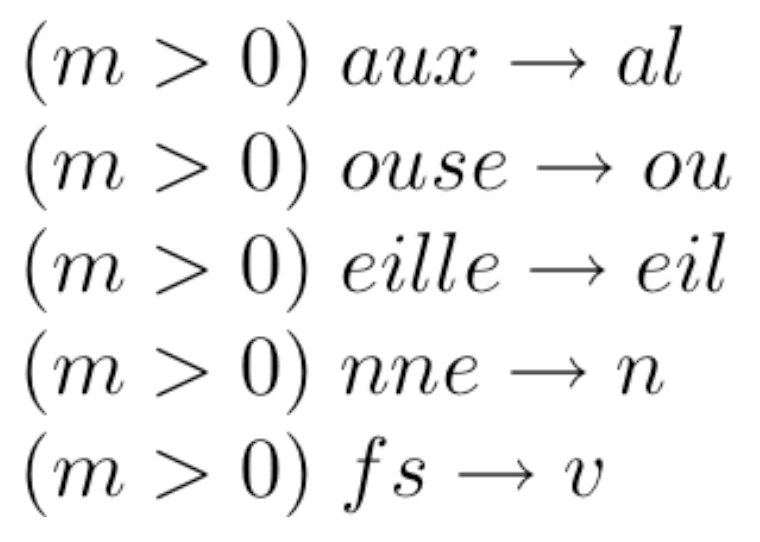
\includegraphics[width=5cm]{stemming_regels_frans}
  \captionof{figure}{Voorbeeld van stemming regels in het Frans}
\end{center}
%%
Tenslotte is \textbf{\textit{named entity recognition}} (NER) ook een techniek die men gebruikt bij document pre-processing. Hierbij gaat men entiteiten proberen te detecteren in de tekst en deze labelen. Neem bijvoorbeeld de zin \textit{Yannick heeft zich ingeschreven in de richting Computerwetenschappen aan de Vrije Universiteit Brussel in 2012}. Men kan met NER de entiteiten eruit halen, labelen en volgend resultaat verkrijgen:\\ 
\newline
\textit{$\text{[Yannick]}_{persoon}$ heeft zich ingeschreven in de richting Computerwetenschappen aan de\\ $\text{[Vrije Universiteit Brussel]}_{organisatie}$ in $\text{[2012]}_{tijdsaanduiding}$}
\newline
\newline
Algemeen kan men stellen dat een combinatie van deze technieken alleen maar de uiteindelijke resultaten ten goede komt. Hoe deze gecombineerd kunnen worden, wordt in het onderstaande voorbeeld ge\"illustreerd. 
\begin{center}
  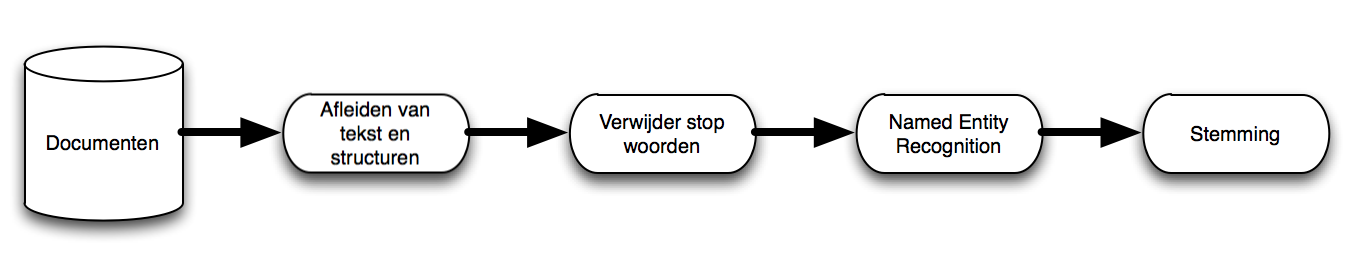
\includegraphics[width=10cm]{document_preprocessing}
  \captionof{figure}{Combinatie van technieken bij document pre-processing}
\end{center}
%
\section{Methoden}\label{Methoden}
Na de document pre-proccesing kunnen we beginnen aan de eigelijke analyse van de dataset. Voor de text mining kunnen we de vector space methode gebruiken.
\subsection{Vector Space Methode}\label{Vector Space Methode}
De vector space methode is een methode waarbij we een document als een vector voorstellen waarbij ieder element overeenkomt met een woord en zijn frequentie in het document. De elementen van de vector worden ook wel features genoemd. Als men concreet een document voorstelt kan men zeggen dat document $j$ voorgesteld wordt door $\textbf{d}_{j}$ met $f_{ij}$ de frequentie van het woord $w_{i}$. Met de frequentie $f_{ij}$ bedoelt men het totaal aantal voorkomens van het woord $w_{i}$ in document $j$. Het aantal verschillende woorden in het document stelt men voor door $n_{w}$, wat eveneens de dimensie is van de vector.
Het document $j$ kan dus als volgt worden voorgesteld:
%
\[ d_{j}  = \begin{bmatrix}
    f_{1j} \\
    f_{2j} \\
    \vdots \\
    f_{n_{w}j} \\
\end{bmatrix}  
\]
%
Een belangrijk inzicht bij het vector space methode is dat een document voorgesteld wordt als een groep van woorden. Er wordt geen rekening gehouden met de volgorde waarin de woorden in het document voorkomen. Vaak ziet men ook dat de vector vaak ijl is en vanwege de grote hoeveelheid aan woorden in een document heel groot. Als we nu niet \'e\'en document maar meerdere documenten nemen en we zeggen dat het aantal documenten gelijk is aan $n_{d}$. Dit resulteert in een matrix waarbij iedere kolom een document voorstelt.
\[
D =
 \stackrel{\mbox{Documenten}}{%
    \begin{bmatrix}
    f_{11} & f_{12} & \cdots & f_{1n_{d}} \\
    f_{21} & f_{22} & \cdots & f_{2n_{d}} \\
    \vdots & \vdots & \ddots & \vdots \\
    f_{n_{w}j} & f_{n_{w}2} & \cdots & f_{n_{w}n_{d}}
    \end{bmatrix}
    }
    & Woorden \]
%
Deze matrix wordt een \textbf{\textit{terms-documents matrix (TDM)}} genoemd. Wanneer men spreekt van een  \textbf{\textit{documents-terms matrix (DTM)}}, spreekt men een getransponeerde terms-documents matrix. Een rij van een DTM stelt dan een document voor.
%
De voorstelling brengt ons dichter bij het vinden van een verband tussen documenten.
We kunnen aan de hand van de euclidische afstand bepalen of documenten gelijkaardig zijn of niet. Stel men heeft twee documenten met een kleine euclidische afstand. Dit wil eigelijk zeggen dat de vectorvoorstelling van de documenten gelijkaardig is. Wat wil zeggen dat de woordfrequenties ongeveer overeen komen en dus bijvoorbeeld de documenten over hetzelfde onderwerp gaan of eenzelfde mening uitdrukken.
%
In de praktijk is gebleken dat documenten vergelijken op basis van woordfrequentie niet altijd de gewenste resultaten oplevert. Vaak is het nog altijd moeilijk om verschillend groepen tussen de documenten te onderscheiden. Daarom kan men nog extra verfijningen toepassen aan de hand van \textbf{\textit{term weighting}} en \textbf{\textit{Latent Semantic Models (LSM)}}.


\subsubsection{Term weighting}\label{Term weighting}

Als men even stil staat bij onze TDM met woordfrequenties, kan men zeggen dat niet elk woord evenveel doorweegt. Een woord dat in alle documenten voorkomt biedt geen of minder waardevolle informatie, dan een woord dat zelden voorkomt. En hierop baseert term weighting zich. Het gaat een wegingsfactor introduceren. Ieder woord krijgt een gewicht toegewezen, dat weergeeft hoe belangrijk het woord is. Neem als voorbeeld een hoop recensies van de film ``Pulp Fiction'' en de woorden ``Pulp'' en ``excellent''. ``Pulp'' is een woord dat voorkomt in de titel van de film en komt ongetwijfeld in elke recensie voor. ``Excellent'' daarentegen is een woord dat enkel maar voorkomt wanneer de recensist de film fantastisch vond, het zal niet in elk document voorkomen en is waardevolle informatie. Term weighting zal dus bij dit voorbeeld ``excellent'' een grotere gewicht toewijzen als ``Pulp''. 
%
De kwantiteit van dit gewicht wordt vaak de \textbf{inverse document frequency  (idf)} genoemd en wordt bepaald aan de hand van volgende formule:
\[w_{i}: idf_{i} = -log_{2}[P(w_{i})] \]
met $P(w_{i})$ de priori probability dat woord $w_{i}$ voorkomt in het document.\\
%
De inverse document frequency geeft het algemeen belang van het woord $w_{i}$ weer. Men kan dit benaderen door het logaritme te nemen van het aantal documenten waar $w_{i}$ in voorkomt en het totaal aantal documenten.
Een andere nuttige kwantiteit is de  \textbf{term frequency} $tf_{ij}$. Deze geeft het belang weer van het woord $w_{i}$ binnen in het document $d_{j}$  en wordt als volgt genoteerd:
\[ tf_{ij} = \frac{f_{ij}}{ \sum_{i=1}^{n_{w}}f_{ij}} \]
%
$tf_{ij}$ wordt berekend door de frequentie, het aantal voorkomens, van een woord $w_{i}$ in document $d_{j}$ te delen door de som van alle woordfrequenties in document $d_{j}$.
Met deze twee kwantiteiten kan men een nieuwe begrip introduceren: de \textbf{tf-idf score}. Wat overeenkomt met het product van tf en idf.
\[ \text{tf-idf score} = tf . idf_{ij} = idf_{i} . tf_{ij} \]
%
De tf-idf matrix bekomt men dan door alle woordfrequenties van het terms-document matrix te vervangen door de tf-idf score.
Deze matrix wordt bijvoorbeeld vaak gebruikt om de gelijkenissen tussen twee documenten te bepalen op basis van cosinusgelijkenis.
%
\subsubsection{Latent Semantic Models}\label{Latent Semantic Models}

Als tweede verfijning van het vector space model, hebben we latent semantic models (LSM). Met LSM probeert men een notie te krijgen van de semantische informatie en meer bepaald het semantisch verband tussen woorden. Bijvoorbeeld als we zoeken naar documenten met het woord ``economie'', willen we ook documenten met ``financi\"en'' terugkrijgen. Voor LSM zijn twee woorden semantisch gerelateerd als ze gebruikt worden in dezelfde context. Met het concrete voorbeeld kunnen we zeggen dat er een semantisch verband is tussen 2 woorden als ze vaak voorkomen in dezelfde documenten.
\newline
Merk op dat bij Latent Semantic Models het wederom belangrijk is dat ieder woord naar \'e\'en concept verwijst.
%
\newline
Analytisch wordt LSM toegepast door \textbf{Singular Value Decomposition (SVD)} toe te passen op de terms-document matrix. SVD is een concept uit de lineaire algebra en zegt dat een matrix A opgesplitst kan worden als een product van matrixen namelijk \\
\[A = U\Sigma V^T \]
De reductie van de dimensie gebeurt aan de hand van volgend principe
%
%afbeelding van SVD in latex
\newcommand{\vect}{\mathbf}
\newcommand{\nul}{\operatorname{Nul}}
\newcommand{\col}{\operatorname{Kolommen }}
\newcommand{\row}{\operatorname{Rijen}}
\[
   A= U\Sigma V^T=
  \begin{matrix}
    \underbrace{\left[\begin{matrix}\vect u_1 & \vect u_2 & \dots & \vect u_r\end{matrix}\right.}& 
    \underbrace{\left.\begin{matrix}\vect u_{r+1} & \dots &  \vect u_m\end{matrix}\right]}\\
    \col A & \nul A^T
  \end{matrix}
  \begin{bmatrix}
      \sigma_1 & 0 & \dots & 0 & 0 & \dots & 0 \\
         0 & \sigma_2  & \dots & 0 & 0 & \dots & 0 \\
         \dots& & & & &  \\
         0 & 0 & \dots & \sigma_k  & 0 & \dots & 0 \\
         0 & 0 & \dots & 0 & 0 & \dots & 0 \\
         \dots& & & & &  \\
         0 & 0 & \dots & 0 & 0 & \dots & 0 
  \end{bmatrix}
  \begin{bmatrix}
    \vect v_1^T \\ \vect v_2^T \\ \dots \\ \vect v_r^T \\
    \vect v_{r+1}^T \\ \dots \\ \vect v_n^T
  \end{bmatrix}
  \begin{matrix}
    \left.\vphantom{\begin{bmatrix}
       \vect v_1^T \\ \vect v_2^T \\ \dots \\ \vect v_r^T 
       \end{bmatrix}}\right\}\row A \\ 
    \left.\vphantom{\begin{bmatrix}
      \vect v_{r+1}^T \\ \dots \\ \vect v_n^T 
    \end{bmatrix}}\right\}\nul A
  \end{matrix}
\] 
\newline
U is de unitaire matrix waarbij men $u_1, u_2, ... , u_n$ de linker singuliere vectors noemt. Deze stellen een document met zijn features voor. $V^T$ is de geconjugeerde getransponeerde matrix van V. $v_1, v_2, ... , v_n$ noemt men de rechter singuliere vectors en stellen de woorden met hun features over alle documenten voor. $\Sigma$ is diagonaal matrix met singuliere waarden $\sigma_1,\sigma_2,..,\sigma_n$'  op de diagonaal. De reductie van een term-document matrix naar een dimensie van $K$ gebeurt door de hoogste $K$ singuliere waarden te nemen in $\Sigma$ met de overeenkomstige singuliere vectoren uit $U$ en $V$.    
Doordat men de dimensionaliteit van de vectoren kan beperken door semantisch gelijkaardige woorden bijeen te voegen. Laat dit het toe om een soort van context groepen te cre\"eren en zo een zeker inzicht te krijgen in de dataset. Het is dan ook gebleken dat SVD toepassen een zeer nuttige eerste stap is bij text mining \cite{maas2011learning} omdat men nieuwe meer effici\"ente features krijgt. De nieuwe features geven meer duidelijkheid en inzicht en kunnen dienen als input voor een machine learning algoritme dat probeert text te analyseren bijvoorbeeld bij classificatie of sentiment prediction.

\chapter{Conclusie}\label{Conclusie}

Voor deze bachelorproef gingen we onderzoeken of de werkwijzen voor engelstalige gevoelsanalyse ook toepasbaar zijn voor nederlandstalige gevoelsanalyse en proberen we deze verschillen beter te specificeren. We hebben getracht om aan de hand van een experimentele analyse hier een antwoord op te vinden.
In de experimentele analyse hebben we een algemeen beeld proberen te vormen over Nederlandse gevoelsanalyse. We hebben in \ref{Engelse gevoelsanalyse versus Nederlandse Gevoelsanalyse} een directe vergelijking gemaakt met Engelse gevoelsanalyse. In deze vergelijking zagen we dat Engelse gevoelsanalyse in het algemeen beter presteerde dan Nederlandse gevoelsanalyse, maar dat voor beide gevoelsanalyses er goede resultaten werden behaald. En de technieken voor Engelse gevoelsanalyse wel degelijk overdraagbaar zijn naar Nederlandse gevoelsanalyse. We zijn mogelijke oorzaken van die betere prestatie voor het Engels gaan onderzoeken. Hieruit konden we besluiten dat de impact van de hoeveelheid woorden (data) in een tekst een rol spelen in de prestatie. We zagen een duidelijk prestatie voordeel bij de Engelse dataset met langere woorden. Dit bevestigd nogmaals dat een goed presterende gevoelsanalyse met de huidige technieken enkel mogelijk is voor meer substanti\"ele teksten, en moeilijk tot onmogelijk voor kortere stukken tekst.\\
Ook zagen we in beide analyseresultaten dezelfde trends. Zo zagen we voor beide talen de Naive Bayes Classifier in combinatie met het verwijderen van stopwoorden, Term weighting en Bigrams als beste techniek en zagen we dezelfde prestatieverschillen tussen de algoritmen mee overgaan van het Engels naar het Nederlands.\\

Vervolgens hebben we classificatie onderzocht op basis van geannoteerde woordenlijsten van gevoelens. Hier hadden we voor de Nederlandse woordenlijsten, een vertaling gebruikt van de Engelse woordenlijsten. Hier konden we besluiten dat Engels woordenlijsten niet transparant vertaald kunnen worden naar het Nederlands en de classificatie onvoldoende presteert. We zagen hier deels de oorzaak lag bij een andere woordenschat, leenwoorden, schrijffouten, internetslang en uitgesmeerde woorden. In verder onderzoek kan men deels deze invloeden wegnemen door de woordenlijsten zelf samen te stellen op basis van een Nederlandse dataset en hier de prestatie van te onderzoeken. Een andere opvallende bevinding uit dit experiment is de opvallende overeenkomst van negatieve engelstalige woorden in onze Nederlandse dataset. Dit kan ook een gevolg zijn van de herkomst van onze Nederlandse dataset (een ‘internetpubliek’ dat onder andere veel gebruikt maakt van anglicismen).\\

Als laatste hebben we de invloed van jargon onderzocht bij Nederlandse gevoelsanalyse. Hier zagen we dat wanneer men een classifier traint voor een bepaald jargon deze ook het beste presteert voor dat jargon. Ook zagen we dat een algemeen concept, het onderscheiden van een positieve en negatieve opinie, kan aangenomen worden door de classifier, desondanks het jargon in de datasets.\\

We hebben aangetoond dat technieken voor gevoelsanalyse grotendeels overdraagbaar zijn, al is het belangrijk om rekening te houden met het feit dat technieken die afhangen van uitgebreid geannoteerde woordenlijsten vaak niet rechtstreeks te vertalen zijn. Voor deze aanpakken is het dus nodig om per taal aangepaste woordenlijsten op te stellen. Maar gezien de goede prestaties van technieken die zonder deze lijsten kunnen werken, kunnen we stellen dat het vaak interessanter is om te investeren in de ontwikkeling van een goede herbruikbare leertechniek in plaats van een uitgebreide geannoteerde woordenlijst per taal.

\end{document}

